The margin of error range is narrowed by selecting a target range and applying corrective coefficients to the reported solar array dust factor in combination with revised performance degradation factors pertaining to shadowing and other losses. Table \ref{tab:target-error-margins} presents the adjustment coefficients that were iteratively obtained. Shadowing and other losses was constrained based on the assumption that they cumulatively range from 5\% to 7\%.

Negative error margin values correspond to over-estimated daily energy predictions, hence the -10\%/+25\% range is preferred in order to limit over-estimations. From the possible combinations of dust factor adjustment with shadowing and other losses, the option with the smallest dust factor adjustment is preferred so to not rely on large changes of the reported duct factor to calibrate Equation \ref{eq:SA_energy}.

\begin{table}[h]
\centering
\caption{Combination of shadowing and other losses with solar array dust factor adjustment coefficients to obtain different error margin ranges. }
\label{tab:target-error-margins}
\begin{tabular}{|c|c|c|}
\hline
\textbf{\begin{tabular}[c]{@{}c@{}}Error\\ Margins\\ Ranges\end{tabular}} & \textbf{\begin{tabular}[c]{@{}c@{}}Shadowing\\ and\\ Other Losses\end{tabular}} & \textbf{\begin{tabular}[c]{@{}c@{}}Solar Array\\ Dust Factor\\ Adjustment\end{tabular}} \\ \hline
\multirow{3}{*}{-20\% / +18\%} & 5\% & 7.5\% \\ \cline{2-3}
 & 6\% & 5.5\% \\ \cline{2-3}
 & 7\% & 3.5\% \\ \hhline{|=|=|=|}
\multirow{3}{*}{-15\% / +21\%} & 5\% & 10.3\% \\ \cline{2-3}
 & 6\% & 8.3\% \\ \cline{2-3}
 & 7\% & 6.3\% \\ \hhline{|=|=|=|}
\multirow{3}{*}{-14\% / +22\%} & 5\% & 10.8\% \\ \cline{2-3}
 & 6\% & 8.8\% \\ \cline{2-3}
 & 7\% & 6.3\% \\ \hhline{|=|=|=|}
\multirow{3}{*}{-13\% / +23\%} & 5\% & 11.4\% \\ \cline{2-3}
 & 6\% & 9.4\% \\ \cline{2-3}
 & 7\% & 7.4\% \\ \hhline{|=|=|=|}
\multirow{3}{*}{-12\% / +23\%} & 5\% & 11.9\% \\ \cline{2-3}
 & 6\% & 9.9\% \\ \cline{2-3}
 & 7\% & 7.9\% \\ \hhline{|=|=|=|}
\multirow{3}{*}{-11\% / +24\%} & 5\% & 12.5\% \\ \cline{2-3}
 & 6\% & 10.5\% \\ \cline{2-3}
 & 7\% & 8.5\% \\ \hhline{|=|=|=|}
\multirow{3}{*}{-10\% / +25\%} & 5\% & 13.1\% \\ \cline{2-3}
 & 6\% & 11.1\% \\ \cline{2-3}
 & 7\% & 9.1\% \\ \hline
\end{tabular}
\end{table}


\clearpage
Applying a 9.1\% dust factor adjustment coupled with a 7\% shadowing and other losses results in the adjusted divergences presented in Figure \ref{fig:plot:mer-energy-prediction-divergences-adjusted}:

\begin{figure}[h]
  \centering
  \hypersetup{linkcolor=captionTextColor}
  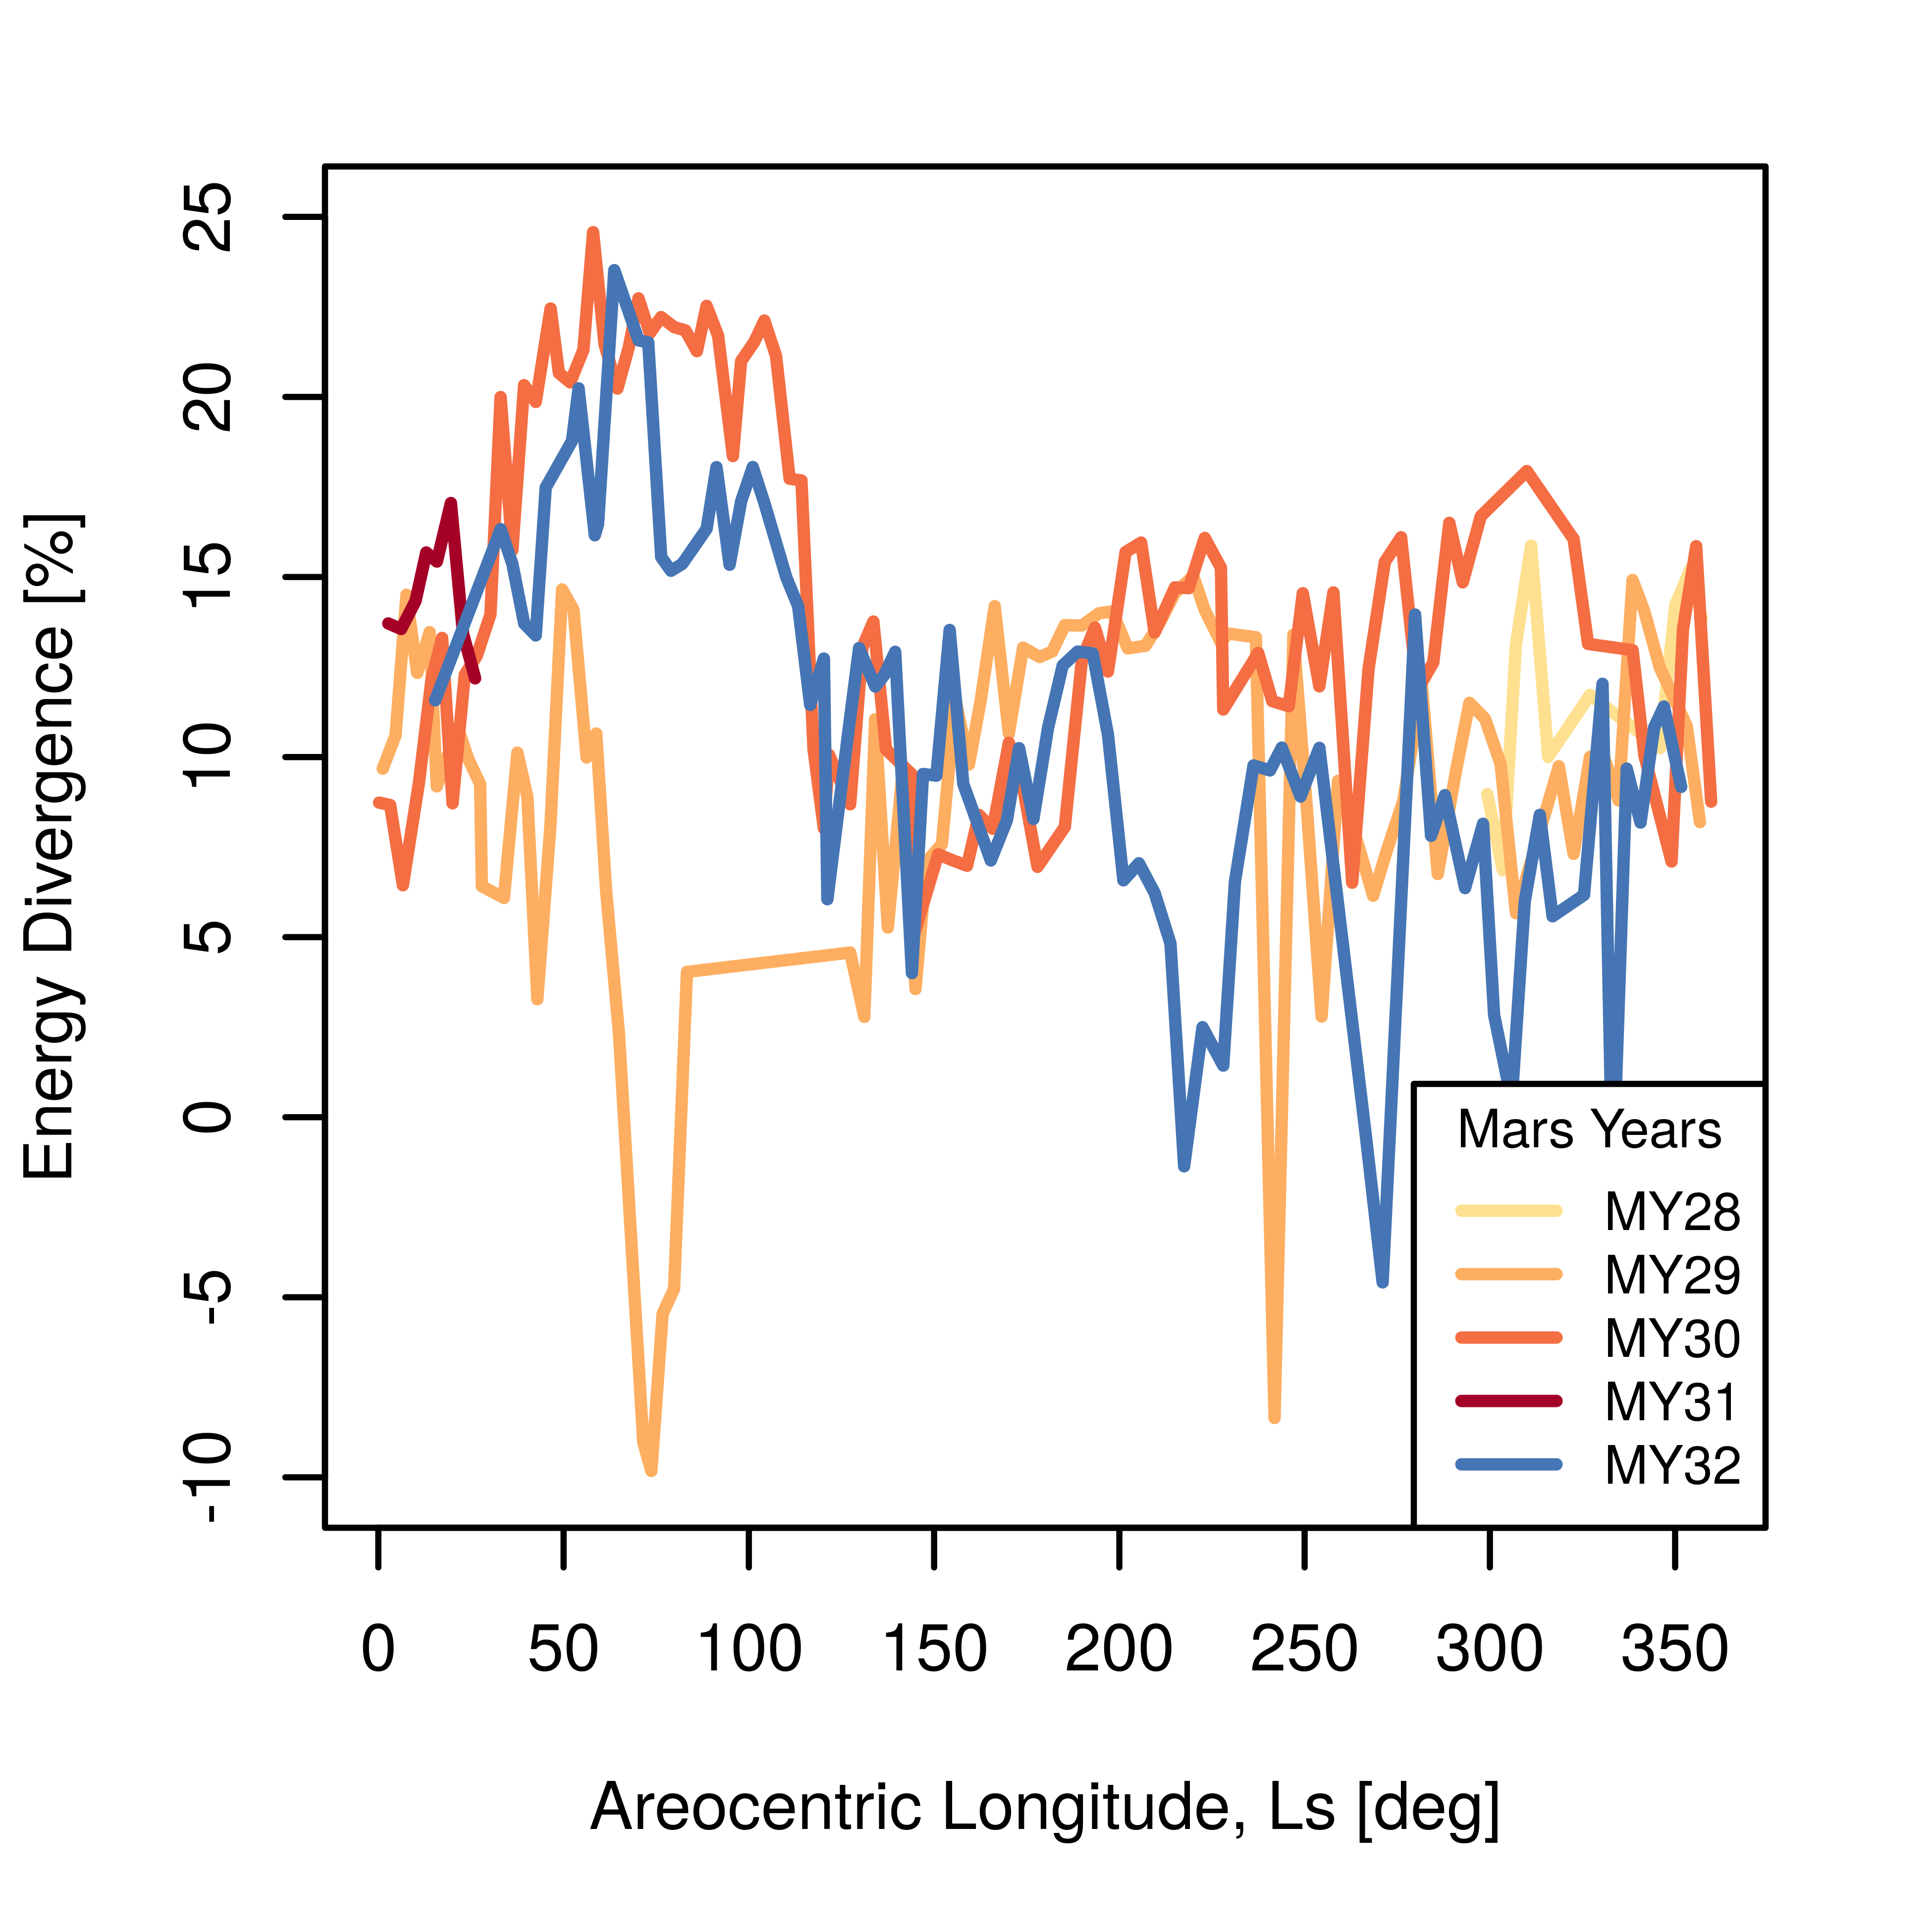
\includegraphics[width=0.8\linewidth]{sections/appendix/B/plots/energy-prediction-divergences-from-my28-to-my32-adjusted.png}\\
  \caption[Adjusted divergences from measured \ac{MER} Opportunity PV energy production]
          {Adjusted divergences from measured \ac{MER} Opportunity PV energy production.}
  \label{fig:plot:mer-energy-prediction-divergences-adjusted}
\end{figure}
